\vspace*{-0.4cm}
\section*{Pregunta 1}

\begin{enumerate}
    \item A continuación se presenta el ruteo correspondiente:
\begin{center}
    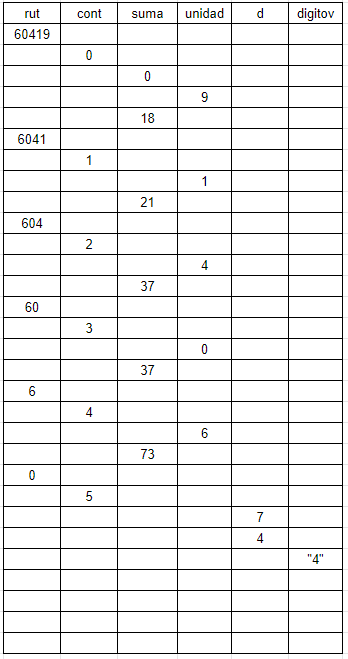
\includegraphics[scale=0.84]{Imagenes/ruteo_pauta}
\end{center}

    El programa imprime \texttt{4}.

    \item El código calculaba el dígito verificador del RUT. También era aceptable responder que, en base a cierto numero, este programa entrega un caracter que podría ser un dígito o una k.

\end{enumerate}

\newpage
\section*{Pregunta 2}

A continuación se presenta una forma posible de resolver el problema propuesto:
\lstinputlisting[
    style  = mypy,
    caption= \texttt{biblioteca.py}]{Code/p2.py}

\newpage
\section*{Pregunta 3}

A continuación se presenta una forma posible de resolver el problema propuesto:
\lstinputlisting[
    style  = mypy,
    caption= \texttt{tepyton.py}]{Code/p3.py}